% -----------------------------------------------
% Template for SMAC SMC 2013
% adapted and corrected from the template for SMC 2012, which was adapted from that of SMC 2011
% further updated for TENOR 2015, 2016 and 2017
% -----------------------------------------------

\documentclass{article}
\usepackage{tenor2017}
\usepackage{ifpdf}
\usepackage[english]{babel}
\usepackage{balance}
\usepackage{courier}

%%%%%%%%%%%%%%%%%%%%%%%% Some useful packages %%%%%%%%%%%%%%%%%%%%%%%%%%%%%%%
%%%%%%%%%%%%%%%%%%%%%%%% See related documentation %%%%%%%%%%%%%%%%%%%%%%%%%%
%\usepackage{amsmath} % popular packages from Am. Math. Soc. Please use the 
%\usepackage{amssymb} % related math environments (split, subequation, cases,
%\usepackage{amsfonts}% multline, etc.)
%\usepackage{bm}      % Bold Math package, defines the command \bf{}
%\usepackage{paralist}% extended list environments
%%subfig.sty is the modern replacement for subfigure.sty. However, subfig.sty 
%%requires and automatically loads caption.sty which overrides class handling 
%%of captions. To prevent this problem, preload caption.sty with caption=false 
%\usepackage[caption=false]{caption}
%\usepackage[font=footnotesize]{subfig}


%user defined variables
\def\papertitle{A Hierarchic Diff Algorithm for Collaborative Music Document Editing}
\def\firstauthor{Christopher Antila}
\def\secondauthor{Jeffrey Trevi\~{n}o}
\def\thirdauthor{Gabriel Weaver}

% adds the automatic
% Saves a lot of ouptut space in PDF... after conversion with the distiller
% Delete if you cannot get PS fonts working on your system.

% pdf-tex settings: detect automatically if run by latex or pdflatex
\newif\ifpdf
\ifx\pdfoutput\relax
\else
   \ifcase\pdfoutput
      \pdffalse
   \else
      \pdftrue
\fi

\ifpdf % compiling with pdflatex
  \usepackage[pdftex,
    pdftitle={\papertitle},
    pdfauthor={\firstauthor, \secondauthor, \thirdauthor},
    bookmarksnumbered, % use section numbers with bookmarks
    pdfstartview=XYZ % start with zoom=100% instead of full screen; 
                     % especially useful if working with a big screen :-)
   ]{hyperref}
  %\pdfcompresslevel=9

  \usepackage[pdftex]{graphicx}
  % declare the path(s) where your graphic files are and their extensions so 
  %you won't have to specify these with every instance of \includegraphics
  \graphicspath{{./figures/}}
  \DeclareGraphicsExtensions{.pdf,.jpeg,.png}

  \usepackage[figure,table]{hypcap}

\else % compiling with latex
  \usepackage[dvips,
    bookmarksnumbered, % use section numbers with bookmarks
    pdfstartview=XYZ % start with zoom=100% instead of full screen
  ]{hyperref}  % hyperrefs are active in the pdf file after conversion

  \usepackage[dvips]{epsfig,graphicx}
  % declare the path(s) where your graphic files are and their extensions so 
  %you won't have to specify these with every instance of \includegraphics
  \graphicspath{{./figures/}}
  \DeclareGraphicsExtensions{.eps}

  \usepackage[figure,table]{hypcap}
\fi

%setup the hyperref package - make the links black without a surrounding frame
\hypersetup{
    colorlinks,%
    citecolor=black,%
    filecolor=black,%
    linkcolor=black,%
    urlcolor=black
}


% Title.
% ------
\title{\papertitle}

% Authors
% Please note that submissions are NOT anonymous, therefore 
% authors' names have to be VISIBLE in your manuscript. 
%
% Single address
% To use with only one author or several with the same address
% ---------------
%\oneauthor
%   {\firstauthor} {Affiliation1 \\ %
%     {\tt \href{mailto:author1@adomain.org}{author1@adomain.org}}}

%Two addresses
%--------------
% \twoauthors
%   {\firstauthor} {Affiliation1 \\ %
%     {\tt \href{mailto:author1@adomain.org}{author1@adomain.org}}}
%   {\secondauthor} {Affiliation2 \\ %
%     {\tt \href{mailto:author2@adomain.org}{author2@adomain.org}}}

% Three addresses
% --------------
 \threeauthors
   {\firstauthor} {nCoda \\ %
     {\tt \href{mailto:christopher@antila.ca}{christopher@antila.ca}}}
   {\secondauthor} {California State University, Monterey Bay \\ %
     {\tt \href{mailto:jtrevino@csumb.edu}{jtrevino@csumb.edu}}}
   {\thirdauthor} { University of Illinois, Urbana-Champaign \\ %
     {\tt \href{mailto:gweaver@illinois.edu}{gweaver@illinois.edu}}}


% ***************************************** the document starts here ***************
\begin{document}
%
\capstartfalse
\maketitle
\capstarttrue
%
\begin{abstract}
We describe an application of hierarchic diff to the collaborative editing of tree-based music representations,
using Zhang and Shasha's tree edit distance algorithm as implemented within the XUDiff tool.
The edit distance between two trees is the minimum number of edit operations necessary to transform one tree into the other.
We consider common operations on the score tree---deleting, changing, and appending tree nodes----to derive a minimal edit sequence,
known as an edit script, and we benchmark the widely used Longest Common Subsequence algorithm against our approach to demonstrate its superior performance.
\end{abstract}
%

\section{Introduction}\label{sec:introduction}
\subsection{The Longest Common Subsequence Algorithm as Default Diff}
Traditional document comparison algorithms, such as in the Unix \texttt{diff} program,
take two sequences of characters as input, and output an edit script to transform one sequence into the other.
An \emph{edit script} consists of a sequence of edit operations (usually insert, delete, and update)
to transform the first sequence relative to some entity---usually characters, words, or lines.
The \emph{edit distance} is the minimum cost the edit script gives for each operation.
The Longest Common Subsequence algorithm and its variants are the most common for computing an edit script and cost.

This approach to document comparison is effective when the inputs are sequences of characters,
and the comparison is displayed in terms of characters, words, or lines of text.
However, many modern file formats use hierarchic object models to encode multiple
levels of meaning (for example, XML or blocks of program code).
As such, purpose-built algorithms are required for hierarchically structured documents.

Consider the following problems that result from using traditional diff tools with hierarchic data.
First, comparing documents with low-level features (like linebreaks in a text file) may not result in
changes that are meaningful in the problem area.
For example, one can generate a ``noisy diff'' in an XML document by changing only linebreaks.
Since linebreaks are not semantically meaningful in XML documents,
the output of a conventional diff algorithm will show a host of apparent changes,
even though no meaningful change occurred.
Second, the very definition of ``sameness'' may change in different contexts.
This is a particular challenge for music, where different criteria are considered when determining
the similarity between musical passages depending on the context.
For example, consider two passages with the same pitches and durations but a different key signature.
While the music sound identically when played,
and music analysts are therefore likely to say the passages are the same,
we can also imagine that someone preparing a critical edition of the score will say the passages are different.
An effective diff on music will support both use cases.
We believe the hierarchic diff presented in this paper lays a foundational prerequisite for such a context-sensitive diff.


\subsection{Collaborative Music Information Requires a Hierarchic Diff}
The noisy diff and contextual definitions of similarity are particular problems when working with music.
From a usability perspective,
we believe that noisy diffs pose an unacceptable barrier to entry to collaborative notation-based tasks.
Although programmers have become accustomed to noisy diffs and the work-arounds they require,
the low adoption rate of computer tools among musicologists and music theorists,
along with the conservative nature of these disciplines,
suggest that a program producing noisy diffs would be perceived as difficult to use,
and therefore not worth the effort.
In addition, the meaning of textually-encoded symbolic music always requires additional interpretation.
Whereas traditional diff algorithms were designed for a one-dimensional sequence of characters,
the immediate meaning of a musical passage is always ambiguous without the context provided by the passage's position in the score hierarchy:
what are the key and metre signatures?
Which instrument is the passage for?
What other instruments are playing at the same time?
The answers to these and other questions may change the meaning of a musical passage entirely.

Yet our primary concern with a music-specific diff algorithm is for use in collaborative systems.
The use of Version Control Systems (VCSes) as a foundation for computer-based collaboration is well known.
From the wide-spread use of VCSes for software development,
the optional use in word processors such as ``Google Docs,''
and even purpose-built tools for legal document preparation,
the ability to track and compare revisions is an important key.
It is in revision comparison that existing free and open source tools have so far failed to meet the needs of musicians,
and it is our intention to remedy this shortcoming with the hierarchic diff implementated for this paper.
We believe that an effective tool for comparing revisions will lead to much greater use of version control for music notation projects,
and thereby enable collaboration on said projects in ways that are currently very difficult.

At the same time, we recognize the importance of making a diff implementation available for computer-driven music research.
In particular, we believe the ability to programmatically compare arbitrary musical passages for their similarity may lead to
ground-breaking research on the use of musical repetition.


\section{Applying The Zhang and Shasha Algorithm}
\subsection{The Zhang and Shasha Algorithm}
Our initial approach uses Zhang and Shasha's tree edit distance algorithm as implemented within the \texttt{XUDiff} tool \cite{Weaver:2013sl}.
The edit distance between two trees is the minimum number of edit operations necessary to transform one tree to another.
The edit operations we consider include deletion, change, and appending of tree nodes.
As before, a sequence of edit operations between two trees is called an \emph{edit script}.

Our proposed approach leverages previous work from other domains, both in industry and in academia.
Within industry, there are proprietary difference engines, such as the \emph{SmartDifferencer} by Semantic Designs,
which compare source code with a variety of edit operations \cite{Designs:qm}.
Within academia, the tree diffing problem has been long studied by theoretical computer science \cite{Bille:2005ec}.
Different algorithms such as subtree hashing,
and even using IDs to align subtrees before computing similarity,
have been studied by researchers such as Chawathe et al. and Cobena et al. \cite{Chawathe:1996jb,Cobena:2002gd}.
We employ the Zhang and Shasha tree difference algorithm to determine the edit distance between trees \cite{Zhang:1989ec,Zhang:1989il}.

One benefit of this approach is that practitioners can choose a preferred level of abstraction
(as defined by level within the tree) with which to summarize a change and define ``similarity.''
As such, we hypothesize that \texttt{XUDiff},
when applied to interpretations of music as encoded in the widely-used hierarchic MEI object model,
will be able to address the problems mentioned above.
Comparing compositions in terms of their meaning as expressed in a hierarchic interpretation of the text and thereby reducing noisy comparisons.


\subsection{Comparative Example}
Consider the case of a simple edit: exchanging a staff's two voices.
That is, the upward-facing stems of voice one become the downward-facing stems of voice two, and vice versa (refer to Figure \ref{fig:voice_swap}).

\begin{figure}[!htb]
\centering
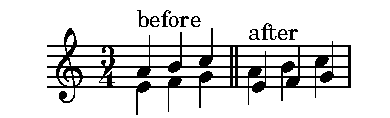
\includegraphics[width=0.8\columnwidth]{layers.pdf}
\caption{An edit that switches the first and second voices in a staff. Stem direction is the only visual difference.}
\label{fig:voice_swap}
\end{figure}

While Common Western Notation displays only a change of stem direction,
a tree-based, hierarchic representation of this musical information must alter both the labeling and succession of elements.
In the MEI XML representation of a music document,
the voice-switch example may be encoded in the following way:

\begin{verbatim}
<staff n="1"> 
    <layer n="1">
        <note pname="a"/>
        <note pname="b"/>
        <note pname="c"/>
    </layer>
    <layer n="2">
        <note pname="e"/>
        <note pname="f"/>
        <note pname="g"/>
    </layer>
</staff>

<!-- ... becomes... -->

<staff n="1">
    <layer n="1">
        <note pname="e"/>
        <note pname="f"/>
        <note pname="g"/>
    </layer>
    <layer n="2">
        <note pname="a"/>
        <note pname="b"/>
        <note pname="c"/>
    </layer>
</staff>
\end{verbatim}


\subsection{Benchmarking LCS against Zhang and Shasha}
How should a diff algorithm represent the described edit?
The Longest Common Subsequence algorithm yields a substantially different result from the Zhang and Shasha Algorithm.
The LCS's line-based comparison yields a diff with an edit distance of 10,
half of which can be attributed to ``noise'' caused by the deletion of the layer element tags (see Figure \ref{fig:lcs_diff}).
On the other hand, the Zhang and Shasha algorithm reports an edit distance of 6 (3 for each layer)
and can aggregate costs across the MEI hierarchy (see Figure \ref{fig:xudiff_diff}).

\begin{figure*}[!htb]
\centering
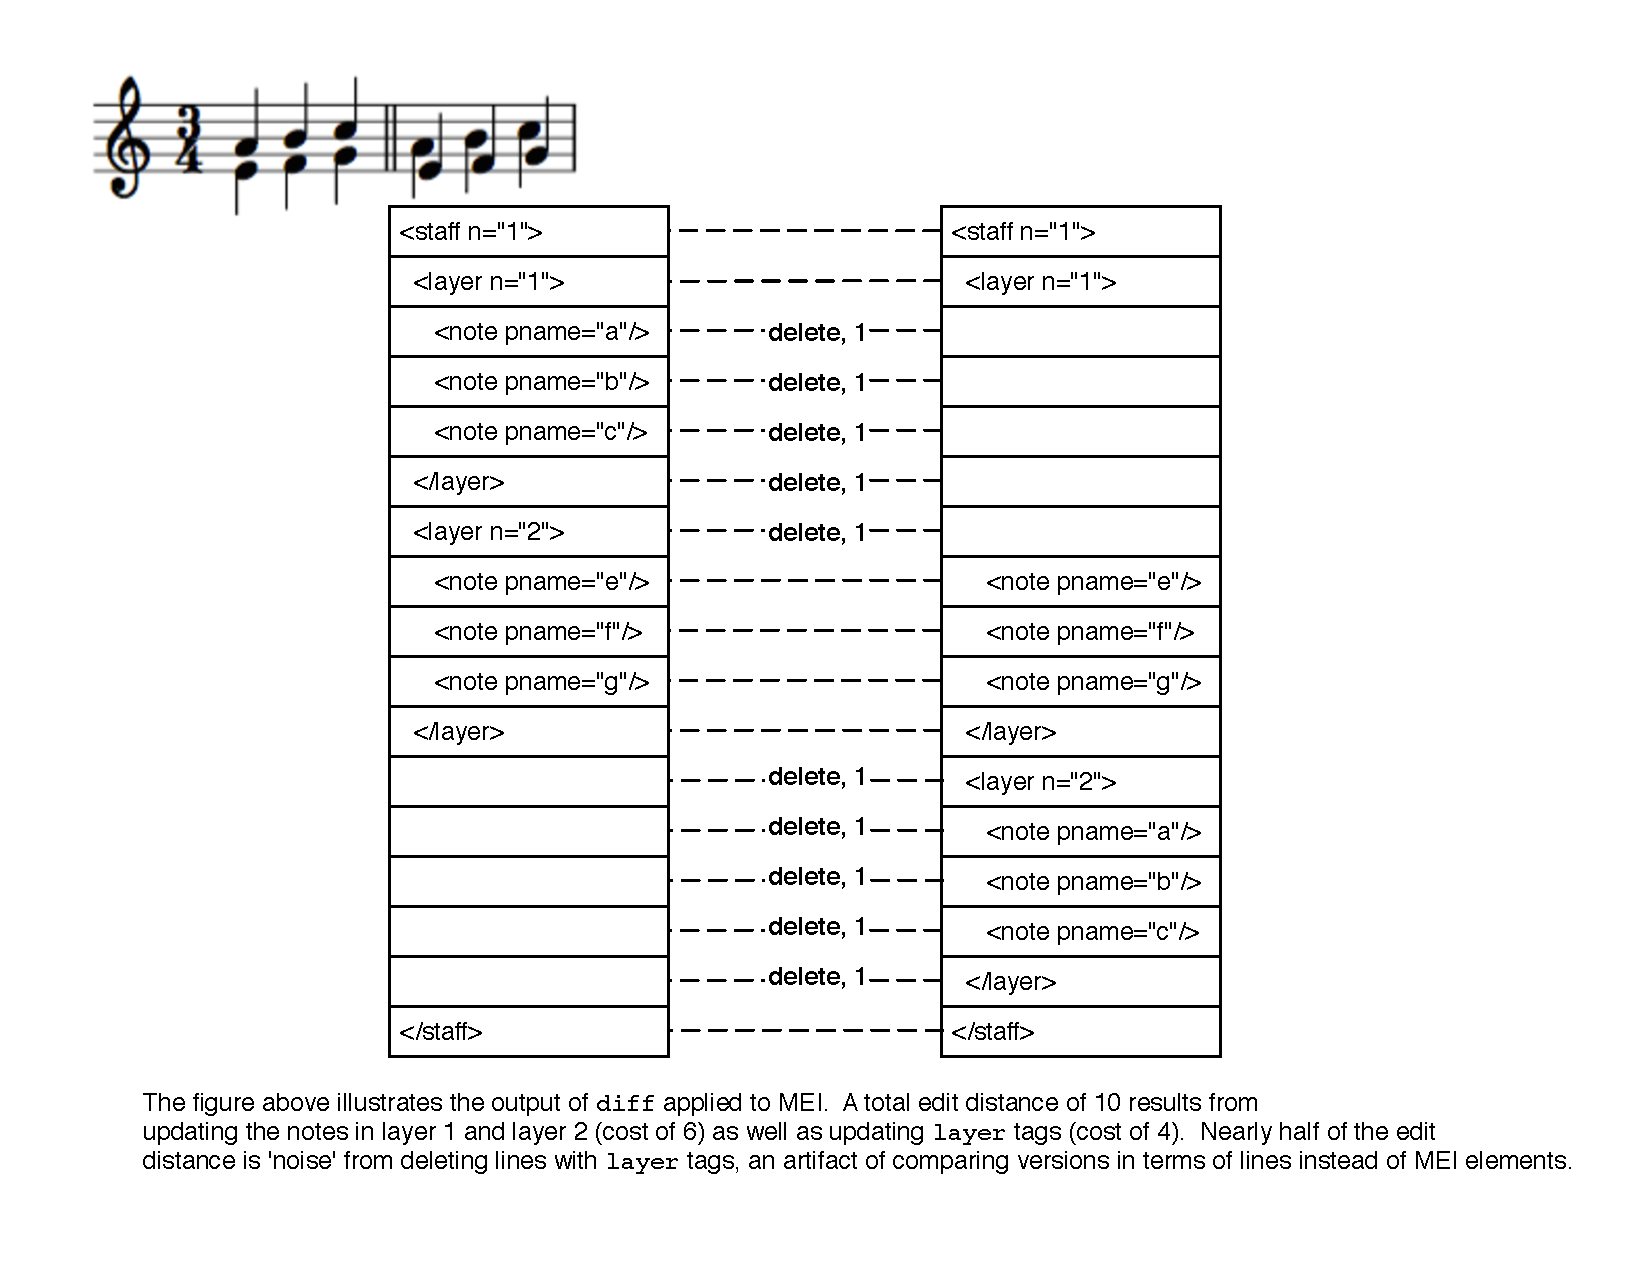
\includegraphics[width=\textwidth]{figure1.pdf}
\caption{The output of \texttt{diff} applied to MEI. A total edit distance of 10 results from updating the notes in layers 1 and 2 (cost of 6), as well as updating \texttt{<layer>} tags (cost of 4). ``Noise'' from layer tag deletion---an artifact of line-based comparison rather than XML element-based comparison--makes up nearly half the edit distance.}
\label{fig:lcs_diff}
\end{figure*}

\begin{figure*}[!htb]
\centering
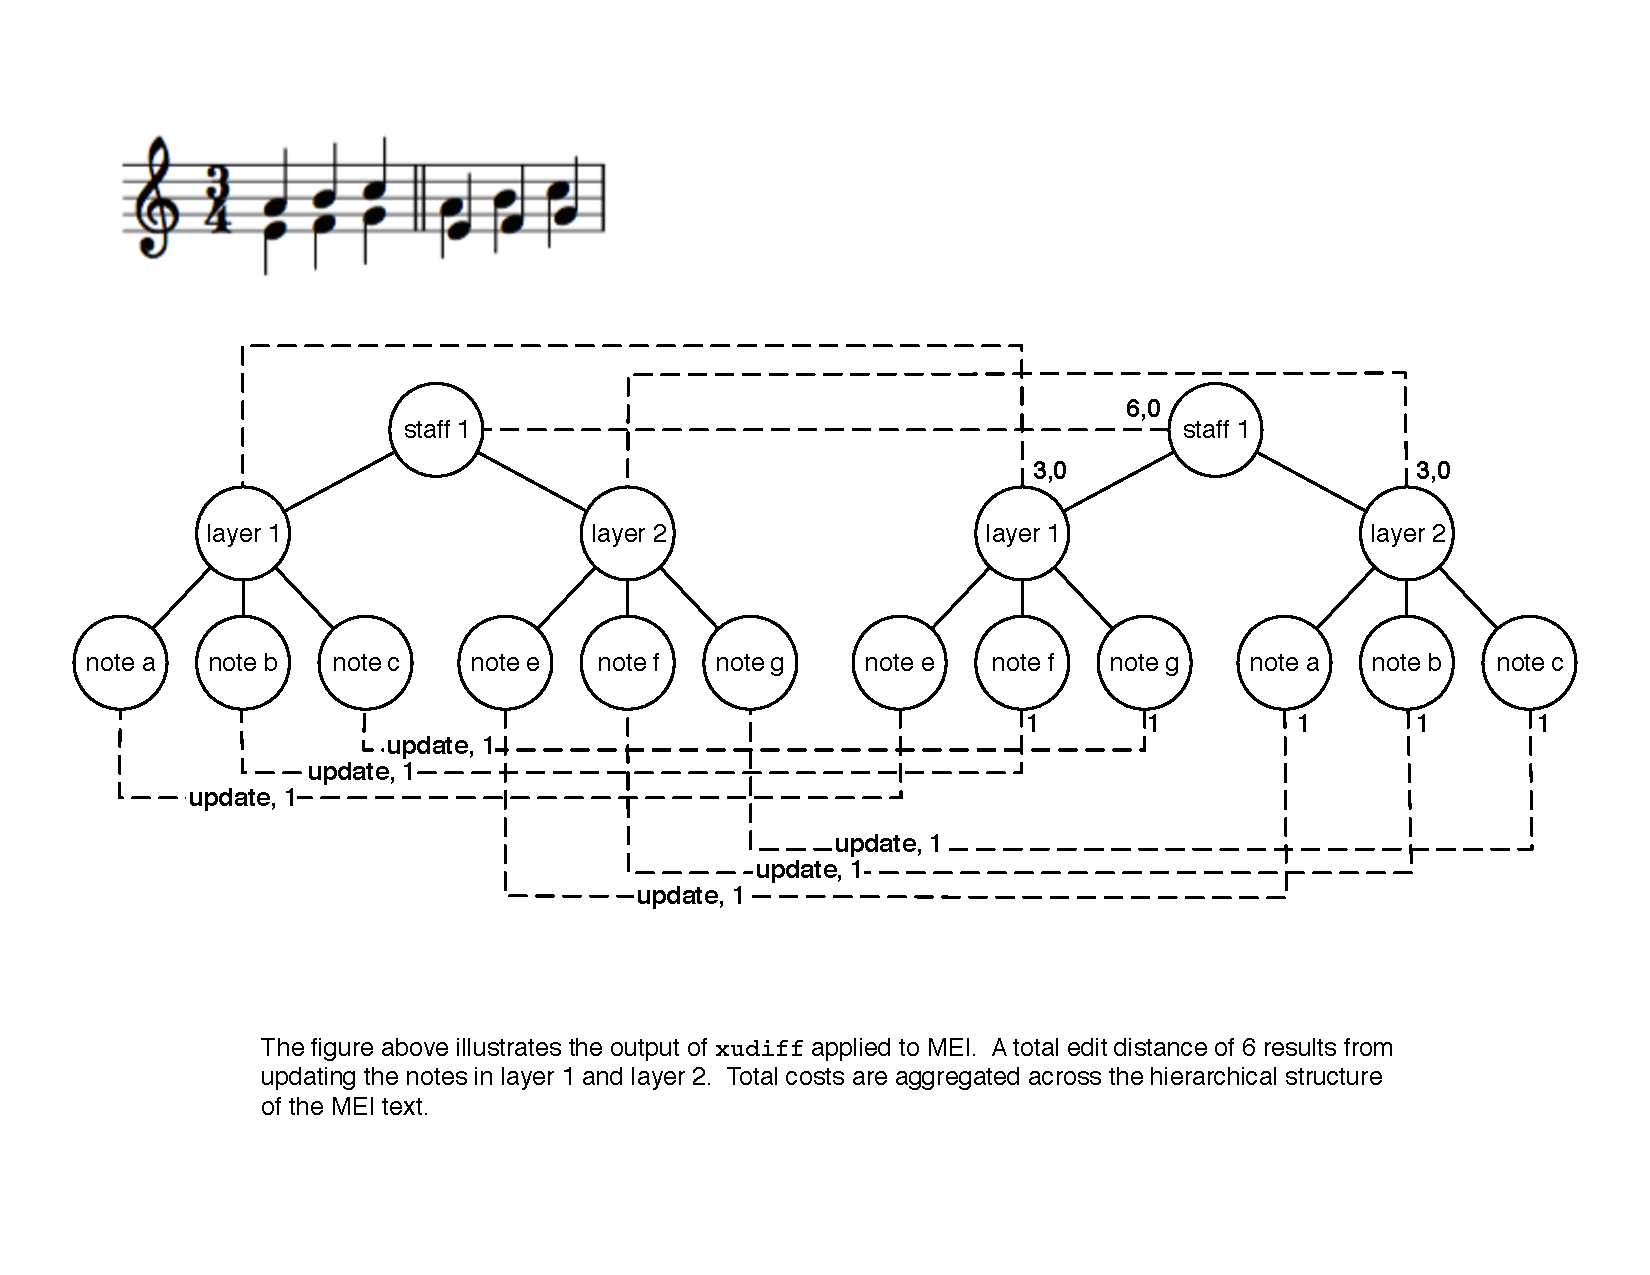
\includegraphics[width=\textwidth]{figure2.pdf}
\caption{The output of \texttt{xudiff} applied to MEI. A total edit distance of 6 results from updating the notes in layers 1 and 2. \texttt{xudiff} aggregates total costs across MEI's hierarchic structure: 3 for each layer and 6 for the staff.}
\label{fig:xudiff_diff}
\end{figure*}

% Jeffrey, please see p. 121 of my thesis for citations
%  What is the related work for this approach in general and
%  specifically to music composition?


\section{Conclusions}
The recently emerged potentials of online collaborative music applications illustrate several ways a robust hierarchic diff algorithm for music can enable newly collaborative musicology, composition, and music education through document utilities \cite{wust2001architectural,Martin:2015pb,McCulloch:2015pd,Flat:aa,Baca:2015xr}.
Yet the commercial presentation of widely used digital engraving tools still conflates the act of sharing with the act of collaboration,
although these remain distinct from each other.
As a recent advertisement for the \emph{Sibelius} engraving program exhorts,
``Collaborate more easily with others and distribute your compositions for the world to hear.
Share scores through email, upload and publish them as sheet music on ScoreExchange.com,
and even share your composition as a video or audio file on YouTube, Facebook, and SoundCloud'' \cite{Avid:to}.
While file exchange between music authors remains a crucial part of musical creativity and collaboration beyond notation,
it is time for engraving software to embrace the potentials of genuinely collaborative music document editing interfaces.

To explore these potential applications, the authors will implement the described algorithm as part of the \emph{nCoda} application,
a free and open source interface for collaborative music document editing.
The algorithm's integration in this project also invites the design of novel user interfaces and diff representation that may take into account the user's music literacy.

%
\begin{acknowledgments}
Research conducted for the \emph{nCoda} project has been supported by Colorado College's SEGway faculty support grant.
\end{acknowledgments}

%%%%%%%%%%%%%%%%%%%%%%%%%%%%%%%%%%%%%%%%%%%%%%%%%%%%%%%%%%%%%%%%%%%%%%%%%%%%%
%bibliography here
\balance
\clearpage
\bibliography{tenor2017diffs}

\end{document}
